\documentclass[aspectratio=169]{beamer}
%\usetheme{CambridgeUS}
%\usecolortheme{beaver}

%\usefonttheme{serif}
%\usepackage{helvet}

\usefonttheme{serif}     % Font theme: serif
%\usepackage{ccfonts}     % Font family: Concrete Math
\usepackage[T1]{fontenc} % Font encoding: T1

\setbeamersize{text margin left=42pt,text margin right=42pt} 
\setbeamertemplate{navigation symbols}{}
\setbeamertemplate{itemize items}[default]

\beamertemplatenavigationsymbolsempty

\definecolor{fore}{RGB}{51,51,51}
\definecolor{back}{RGB}{255, 254, 250}
\definecolor{title}{RGB}{ 255, 15, 0}
\definecolor{links}{RGB}{18, 168, 255}

\setbeamercolor{titlelike}{fg=title}
\setbeamercolor{normal text}{fg=fore,bg=back}
\setbeamercolor{alerted text}{fg=title}
\setbeamercolor{itemize item}{fg=title}
\setbeamercolor{enumerate item}{fg=title}
\hypersetup{colorlinks,urlcolor=links}

% for code https://kbroman.org/blog/2013/10/07/better-looking-latexbeamer-slides/
\usepackage{listings}
\definecolor{keywords}{RGB}{255,0,90}
\definecolor{comments}{RGB}{60,179,113}
\lstset{language=Python,
keywordstyle=color{keywords},
commentstyle=color{comments}emph}

% fonts
\usepackage[sc]{mathpazo}


% title info
\title{\textbf{Health and Equity}
\subtitle{\textbf{GGR424 - Transportation Geography \& Planning}}
\author{Jeff Allen}
\institute{University of Toronto}
\date{March 7, 2022}}




\begin{document}
	
\begin{frame}
	\titlepage	
\end{frame}





\begin{frame}
	
	\textbf{Announcements}
	
	\begin{itemize}
		\item Project Proposal due March 10
	\end{itemize}
	
	
	\textbf{Today}
	
	\begin{itemize}
		\item Health impacts of	transportation (e.g. pollution, noise, physical activity)
		\item How the costs and benefits of transportation are (in)equitably distributed
		
	\end{itemize}
\end{frame}




\begin{frame}
	
	How can urban transportation affect health and well-being?
	
\end{frame}



\begin{frame}
	
	\textbf{Noise}
	
	\begin{figure}
		\centering
		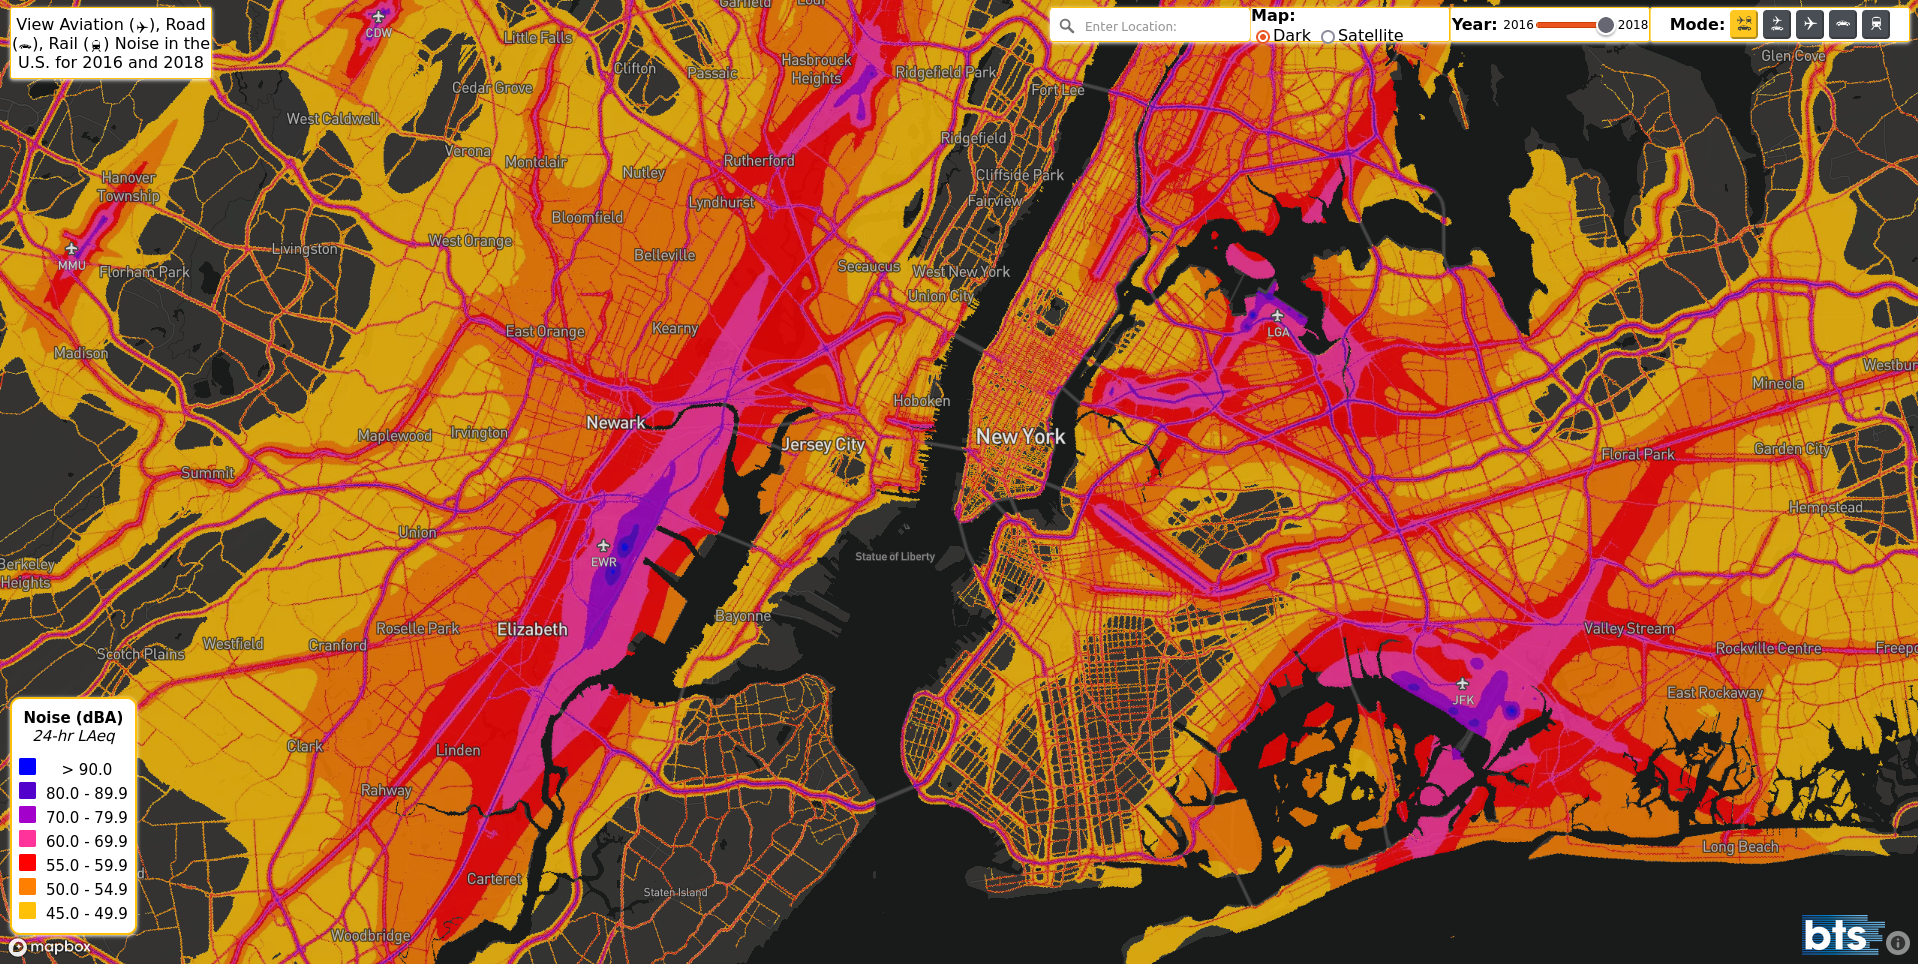
\includegraphics[width=1\linewidth]{images/noise_nyc.png}
	\end{figure}
	\tiny Source: \url{https://maps.dot.gov/BTS/NationalTransportationNoiseMap/}
	
	\vspace{2mm}
	\tiny City report on health impacts of noise \url{https://www.toronto.ca/wp-content/uploads/2017/11/8f98-tph-How-Loud-is-Too-Loud-Health-Impacts-Environmental-Noise.pdf}
	
\end{frame}

% annoyance, innability to concentrate (work school), loss of sleep, increased stress, increased risk of cardiovascular disease






\begin{frame}
	
	\textbf{Air Pollution}
	
	\begin{columns}
		\begin{column}{0.5\textwidth}
			
			
			\begin{figure}
				\centering
				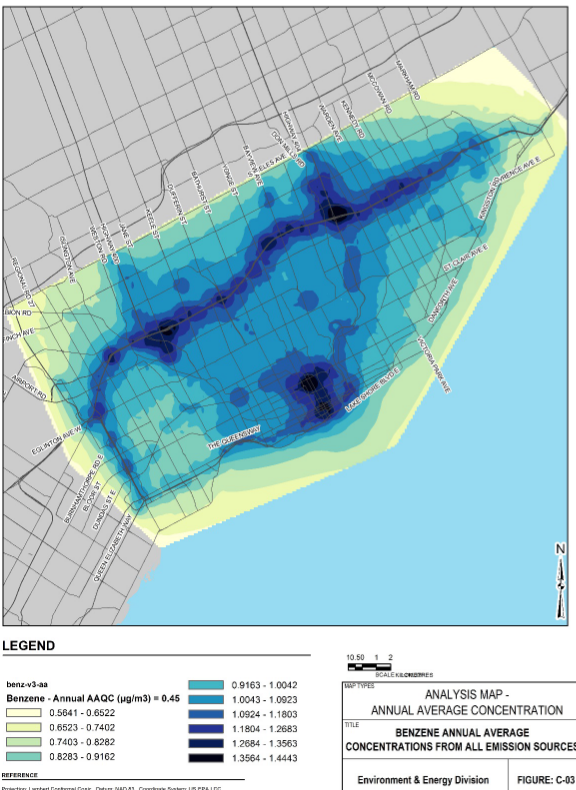
\includegraphics[width=0.8\linewidth]{images/tor_benzene.png}
			\end{figure}
		\end{column}
		
		\begin{column}{0.5\textwidth}
			\begin{figure}
				\centering
				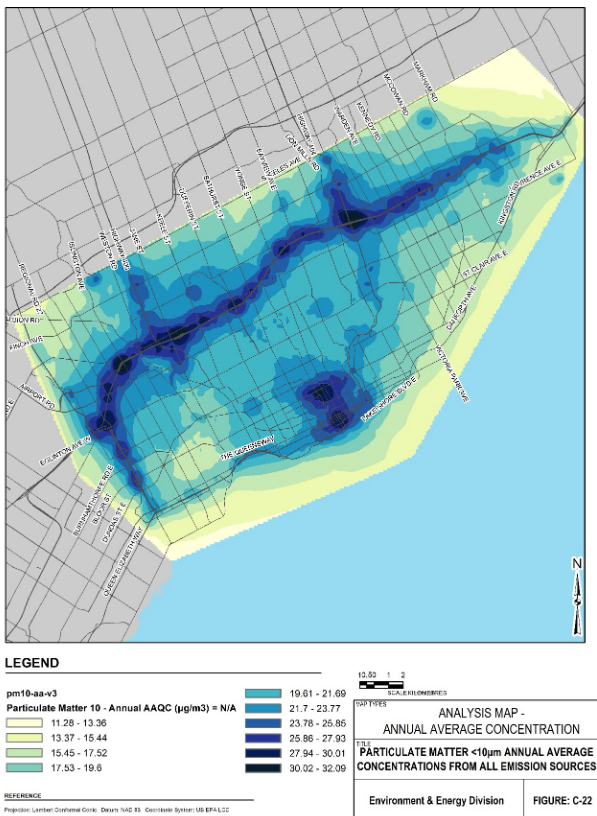
\includegraphics[width=0.8\linewidth]{images/tor_pm10.png}
			\end{figure}
			
		\end{column}

	\end{columns}
	
	\tiny City of Toronto. Avoiding the TRAP: Traffic-Related Air Pollution in Toronto and Options
	for Reducing Exposure. Technical Report. October 2017.: \url{https://www.toronto.ca/legdocs/mmis/2017/hl/bgrd/backgroundfile-108070.pdf}
	
\end{frame}


% pollution - e.g. missed days of activity (i.e. stay inside), asthma, bronchitus, hospitalizations/mortality, etc.






\begin{frame}
	\textbf{Active Travel and Physical Health}
	
	\begin{figure}
		\centering
		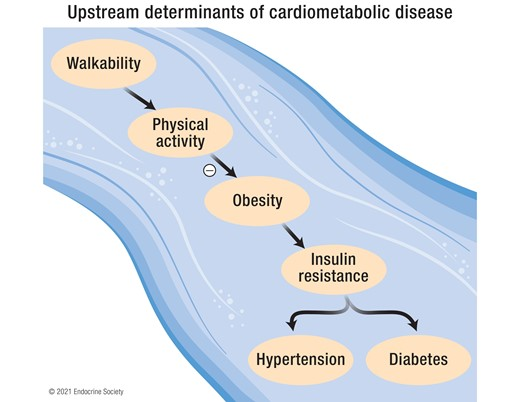
\includegraphics[width=0.6\linewidth]{images/walkability_health}
	\end{figure}
	
	\tiny The weight of place: Built environment correlates of obesity and diabetes \url{https://doi.org/10.1210/endrev/bnac005}
	
\end{frame}

% walkability and physical activity

\begin{frame}
	
	\begin{figure}
		\centering
		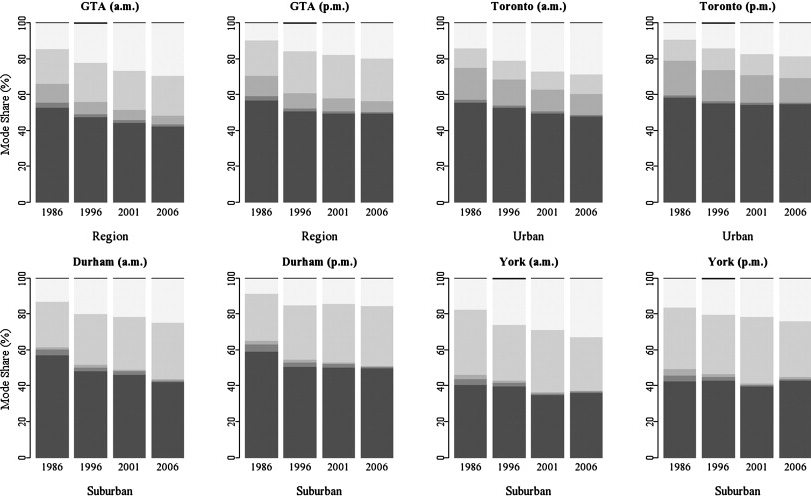
\includegraphics[width=0.9\linewidth]{images/mode_to_school}
	\end{figure}
	
	
	\tiny School travel mode share (\% of trips) by jurisdiction and year (children and youth, 11–13 years of age) in the Greater Toronto Area, Canada (1986–2006).
	
	\tiny\url{https://doi.org/10.1016/j.ypmed.2009.03.001}
	
\end{frame}






\begin{frame}
	
	\textbf{Satisfaction of travel}
	
	\begin{figure}
		\centering
		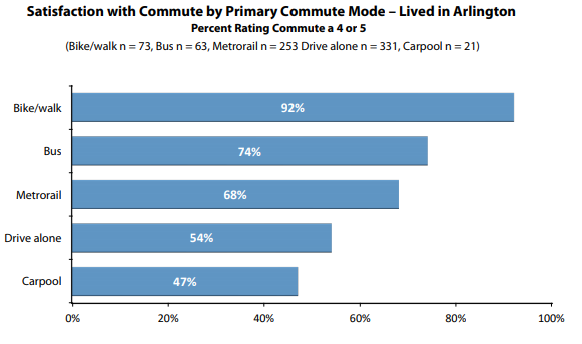
\includegraphics[width=0.7\linewidth]{images/mode_satisfaction.png}
	\end{figure}
	
	\tiny\url{https://mobilitylab.org/2020/09/29/the-pursuit-of-happiness-how-commute-mode-affects-commute-mood/}
	
\end{frame}

% stress of travel, long commutes means less time doing other things


\begin{frame}
	
	\textbf{Long commutes}
	
	\vspace{4mm}
	
	From the 2016 Canadian census:
	
	\begin{itemize}
		\item 9.7\% have a commute greater than 60 minutes
		
		\item 3.5\% have a commute greater than 75 minutes
		
		\item 2.5\% have a commute greater than 90 minutes
	\end{itemize}
	
\end{frame}



% accidents, cars, pedestrians, etc. - but general feelings of safety


\begin{frame}
	
	\textbf{Safety, e.g. Collisions}
	
	\begin{figure}
		\centering
		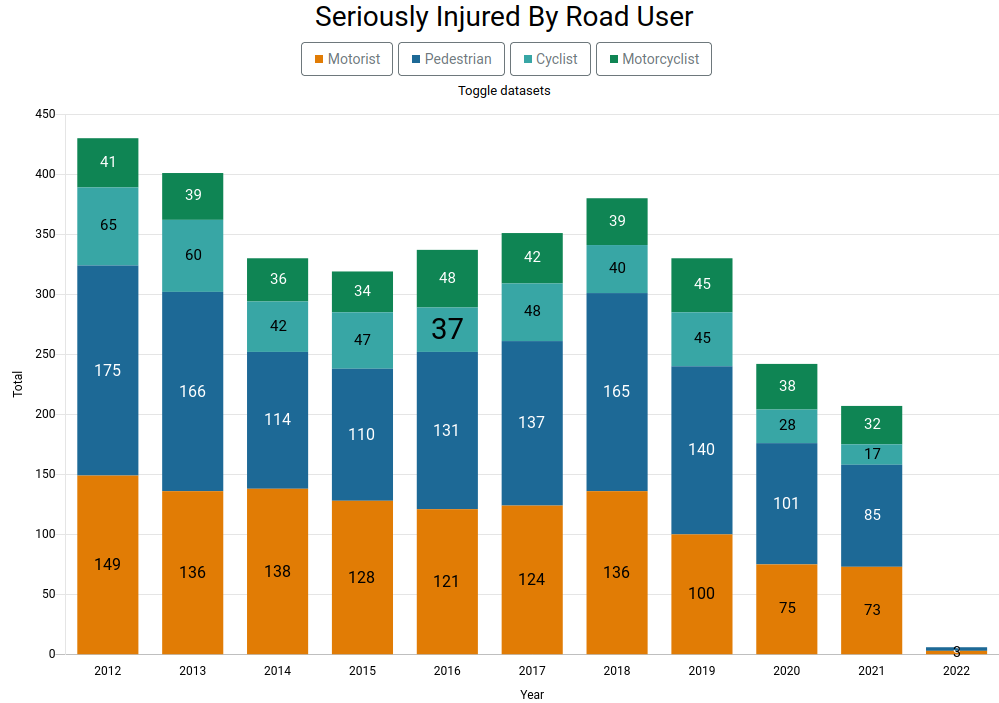
\includegraphics[width=0.7\linewidth]{images/injury_road_tor.png}
	\end{figure}
	
	\tiny \url{https://www.toronto.ca/services-payments/streets-parking-transportation/road-safety/vision-zero/vision-zero-dashboard/seriously-injured-vision-zero/}s
	
\end{frame}




\begin{frame}
	
	\textbf{Safety, e.g. COVID-19}
	
	\begin{figure}
		\centering
		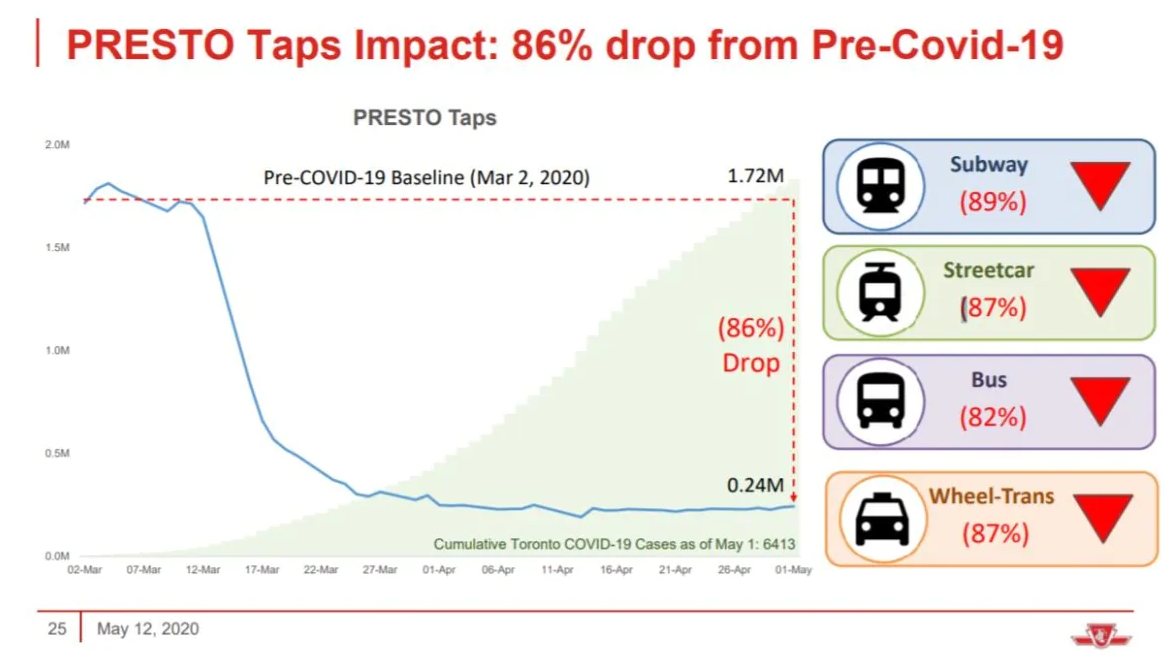
\includegraphics[width=0.94\linewidth]{images/ttc-covid.png}
	\end{figure}
	
		\tiny \url{https://www.cbc.ca/news/canada/toronto/ttc-finances-covid19-1.5569867}
	
\end{frame}




% access to health, groceries, etc. foodbanks

\begin{frame}
	
	\textbf{Accessibility, e.g. to healthy food}
	
	\begin{figure}
		\centering
		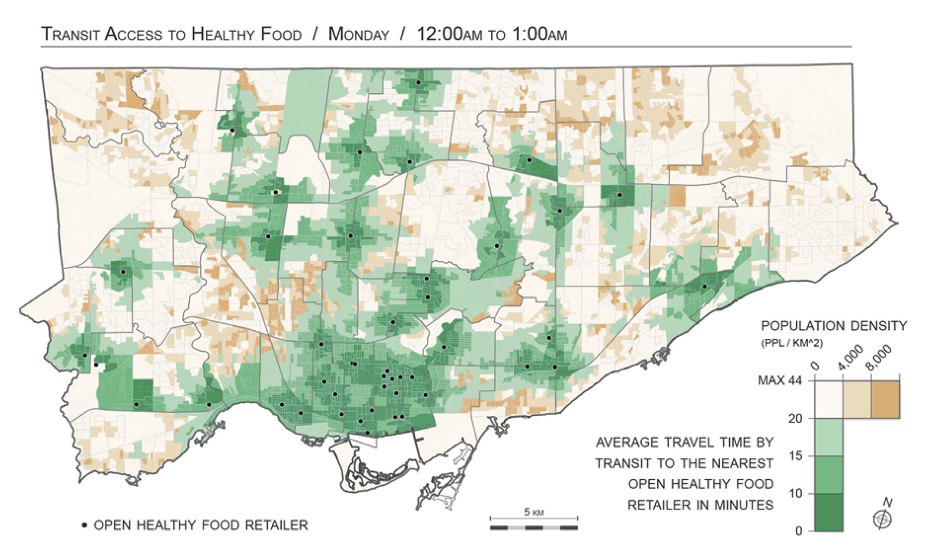
\includegraphics[width=0.94\linewidth]{images/food_midnight.png}
	\end{figure}
	
	\tiny Source: Widener et al (2017) How do changes in the daily food and transportation environments affect grocery store accessibility?
	\url{https://doi.org/10.1016/j.apgeog.2017.03.018}
	
\end{frame}




\begin{frame}
	
	\textbf{Accessibility, e.g. to food banks}
	
	\begin{figure}
		\centering
		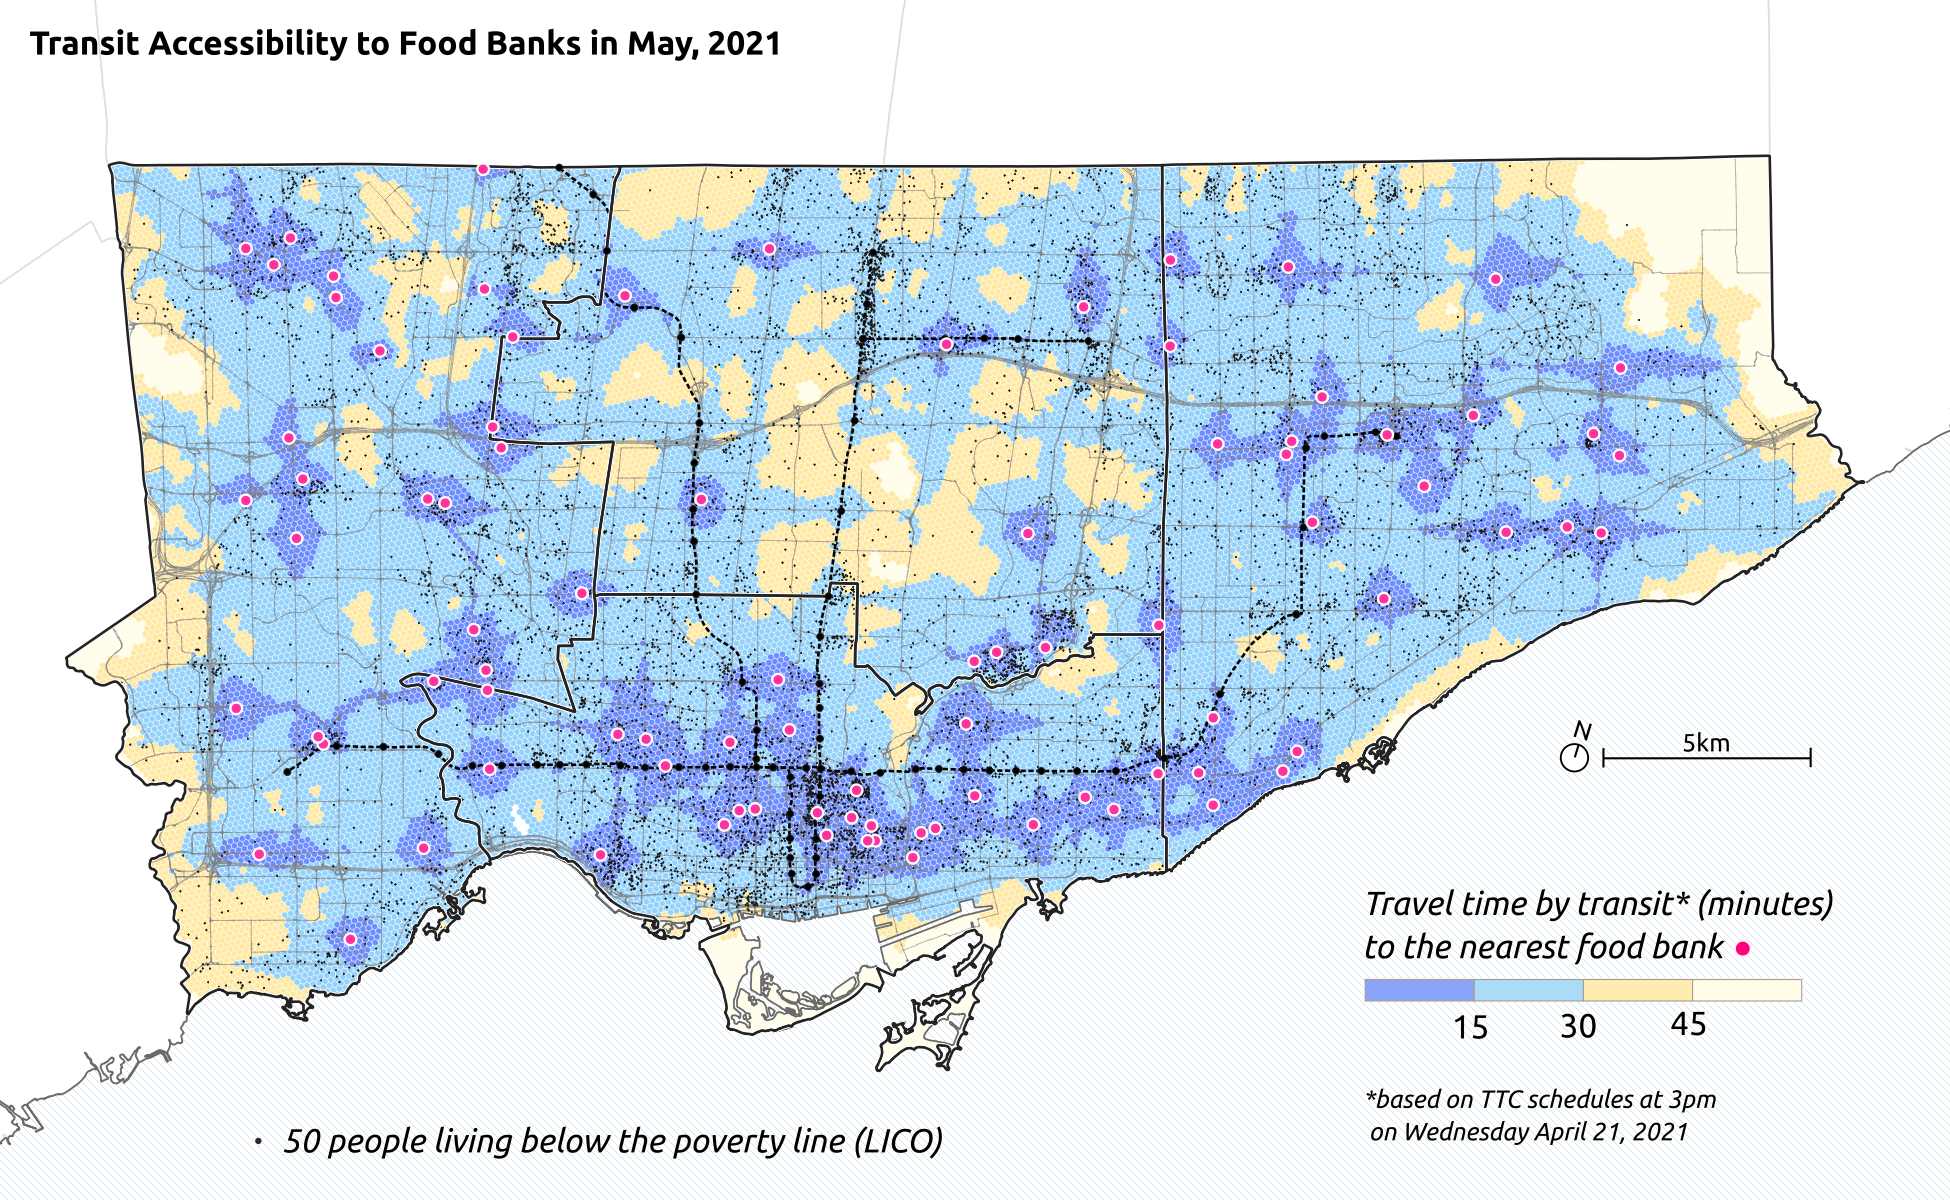
\includegraphics[width=0.94\linewidth]{images/foodbanks_access.png}
	\end{figure}
	
	\tiny 
	\url{https://github.com/SAUSy-Lab/toronto-food-bank-accessibility}
	
\end{frame}




\begin{frame}
	
	\textbf{Transport Equity}
	
	\vspace{4mm}
	
	
	\textit{Equity} generally refers to the fairness with which impacts (i.e. benefits and costs) are distributed 
	
	\vspace{2mm}
	
	Transportation planning decisions can have large and diverse equity
	impacts.
	
	\vspace{2mm}
	
	
	\begin{itemize}	
		\item \textbf{Horizontal Equity} - about the distribution of a resource (e.g. public transit) equally among the overall population
		
		\item \textbf{Vertical Equity} - about the distribution of a resource with focus towards specific groups, often those who are more vulnerable to social or economic exclusion
	\end{itemize}
	
	
\end{frame}




\begin{frame}
	
	\textbf{Transport Equity}
	
	\vspace{4mm}
	
	Dimensions of measuring transport equity
	
	\begin{itemize}	
		\item \textbf{Opportunities} - about how transportation infrastructure and accessibility are (in)equitably distributed
		
		\item \textbf{Exposure} - about inequalities in exposure to pollutants, unsafe travel, etc.
		
		\item \textbf{Outcomes} - about whether there are inequalities in travel behaviour outcomes, e.g. activity participation, commute times, etc.
		
	\end{itemize}
	
	
\end{frame}



\begin{frame}
	
	
	
\end{frame}








\end{document}